\documentclass[11pt]{article}

\usepackage{graphicx} % gere les images 
\usepackage[utf8]{inputenc} % pour les accents
\usepackage{hyperref}
\usepackage[french]{babel}
\usepackage{geometry}

\hypersetup {
	colorlinks=true,
	linkcolor=black,
	urlcolor=red,
	citecolor=green,
	pdftitle={Initiation aux outils de simulation réseaux avec NS-2},
	pdfauthor={Armen,Aurelien},
	pdfsubject={simulation réseau avec NS-2},
	pdfkeywords={NS-2, réseau, nam, esirem, tcp, udp, }
}

\begin{document}

\begin{titlepage}
	\newcommand{\HRule}{\rule{\linewidth}{0.2mm}}     
            
	\begin{figure}[t]
		\begin{minipage}{0.5\textwidth}\large
			\begin{flushleft}
				
\includegraphics[width=0.7\textwidth]{assets/logoEsirem.jpg}
			\end{flushleft}
		\end{minipage}
		\begin{minipage}{0.5\textwidth}\large
			\begin{flushright}
			
\includegraphics[width=0.6\textwidth]{assets/logoUb.jpg}
			\end{flushright}
		\end{minipage}
	\end{figure}
	\textsc{ \\[1cm]}
     
     
	\begin{center}
	\HRule \\
	{\Large   
		Initiation aux outils de simulation réseaux avec NS-2
	}
	\HRule
	\\[0.5cm]
	{\large Compte rendu tp reseau \\}
   \end{center}

	\begin{figure}[h]
		\begin{center}
			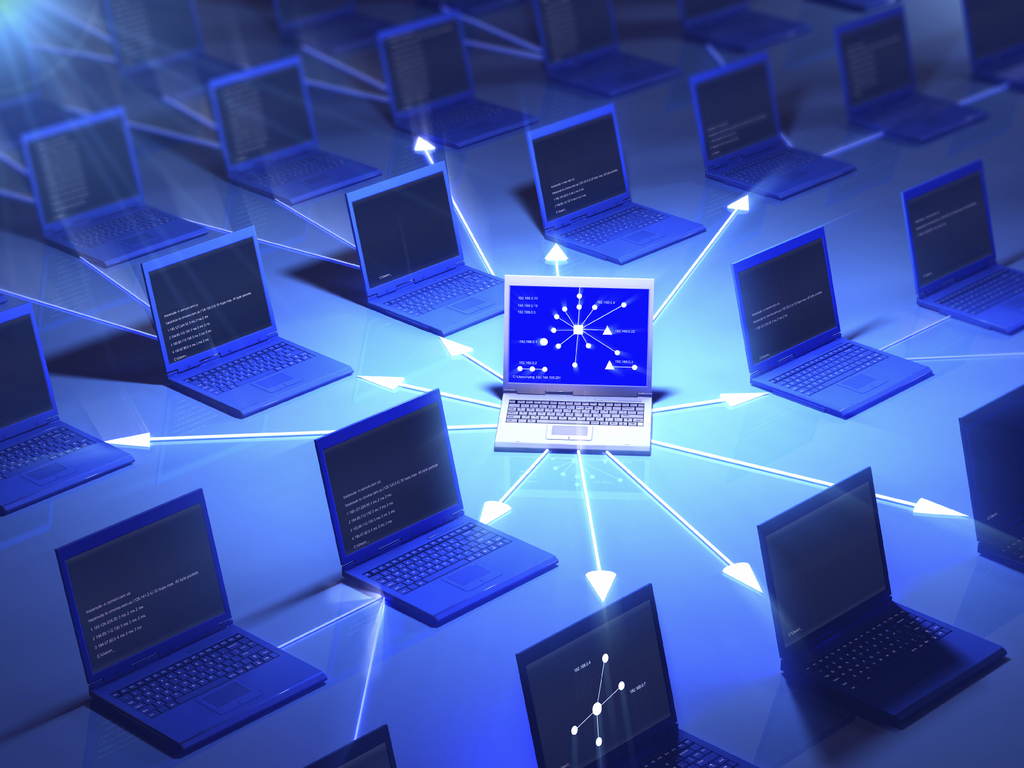
\includegraphics[width=0.4\textwidth]{assets/main.jpg}
		\end{center}
	\end{figure}
        
	\vfill 
	\begin{center}
        \textsc{\large
        	ESIREM \\
			École Supérieure d'Ingénieurs de Recherche en Matériaux et en Infotronique\\       	
			[2cm]
		}
	\end{center}

	\begin{minipage}{0.5\textwidth}
		\begin{flushleft} \large
			\emph{Auteurs:}\\
			Armen Mahmedov \\
			Aurélien Patru
		\end{flushleft}
	\end{minipage}
	~
	\begin{minipage}{0.5\textwidth}
		\begin{flushright}\large
			\emph{Professeurs :} \\
			Nader Mbarek \\
			Ahmad Khalil
		\end{flushright}
	\end{minipage}
        
\end{titlepage}
  
% saut de page  ou   ~ \pagebreak 
\newpage
\strut
\newpage


\tableofcontents


\pagebreak


\section*{Introduction}
\addcontentsline{toc}{section}{Introduction}
Introduction générale 

\pagebreak


% Partie 1
\section{TP 1: Découvert de NS-2 et nam}
[introduction de la partie]

\subsection{Exercice 1: Simulation d'une topologie simple a deux noeuds avec un lien direct}

\subsubsection{Compléter le script}

\subsubsection{Visualisation de la simulation a l'aide de NAM}

\subsubsection{Découvert des fonctionnalités de NAM}

\subsubsection{Utilisation graphique de NAM}


\subsection{Exercice 2: Fonctionnement TCP vs UDP}



[conclusion de la partie]



% Partie 2
\section{TP 2: Protocole de routage de type Vecteur distance et Etat de liens}
[introduction de la partie]

\subsection{Exercice 1: Comparaison des deux protocoles de routage}


\subsection{Exercice 2: Routage et contrôle de congestion TCP}

[conclusion de la partie]

% Partie 3
\section{TP 3: Utilisation de xgraph et NS-2 pour visualiser les performances d'un réseau}
[introduction de la partie]

\subsection{Sous-partie 1}

[conclusion de la partie]




\section*{Conclusion}
\addcontentsline{toc}{section}{Conclusion}
[Conclusion générale]














\end{document}
